\documentclass[main.tex]{subfiles}

\begin{document}
\section{整体设计}
FPGA测试整体设计如下方框图所示。图中白色方框为模块,箭头连线为数据连接线,彩色图形为控制信号。
\begin{figure}[h]
\centering
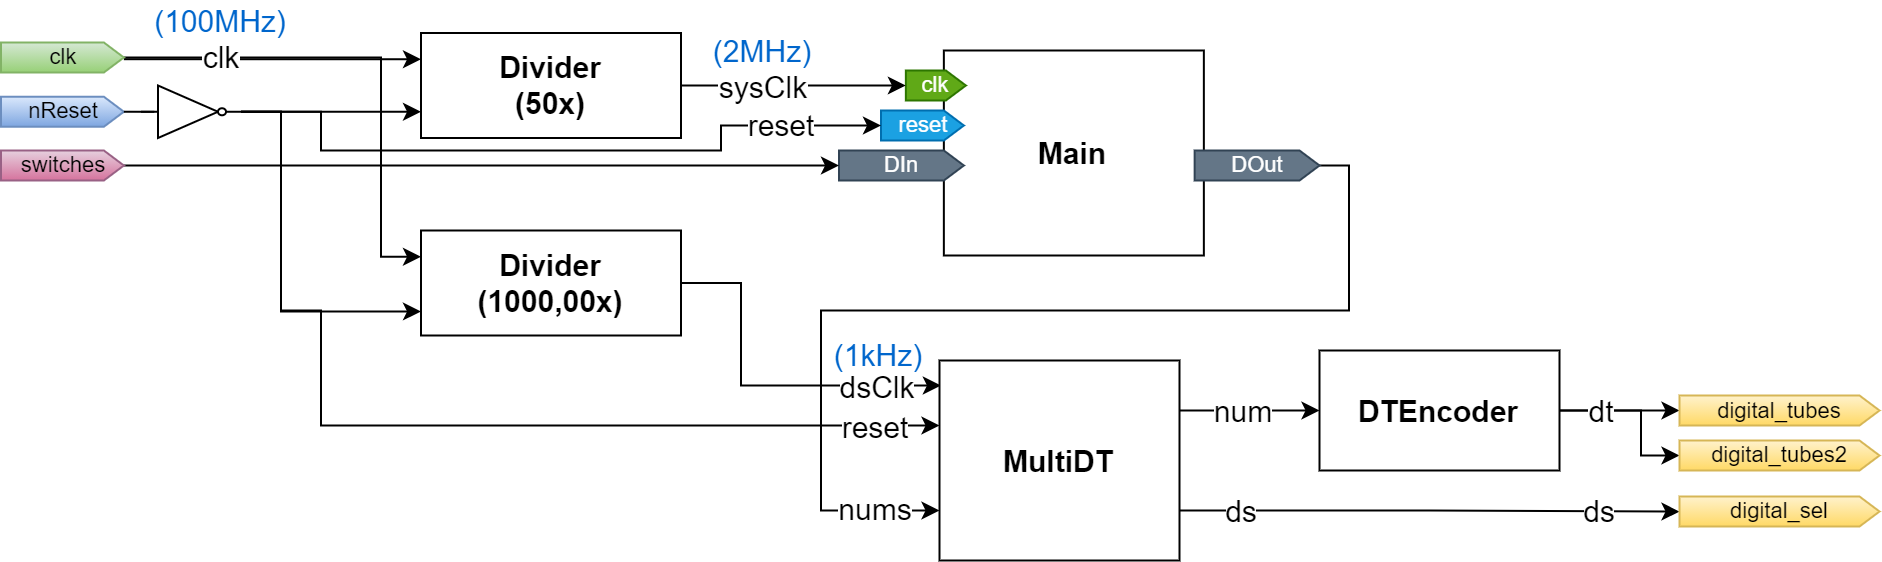
\includegraphics[width=\textwidth]{images/PCOCD-P4-pratical-block.png}
\caption{FPGA测试框图}
\end{figure}

图中$Main$模块与Project3中的整体系统完全一致。

图中的$Divider$为分频器,输入的时钟为100MHz的原始时钟信号。

图中$MultiDT$和$DTEncoder$组成动态数码管,连接到$digital_tubes$、$digital_tubes2$和$digital_sel$驱动八个七段数码管。

图中$nReset$连接到一重置按钮,$switches$连接到32个拨码开关。

\section{模块设计}

Project4的模块设计与Project3的模块设计变化很小,故此简单使用文字描述其变化。

\paragraph{新增分频器、动态数码管控制模块}
新增的分频器、动态数码管控制模块均是数字逻辑实验中学习、实践过的模块,且并非本课程的重点,故此不在此详细说明,仅简单说明其特性。

\subparagraph{分频器}
分频器内部有一个寄存器用于计数,只有输入的时钟信号$clkIn$变化指定次数后,才会触发输出时钟信号$clkOut$的一次变化。

\subparagraph{动态数码管控制模块}
动态数码管指的是,每个数码管在指定的时间下点亮一小段时间,数码管使能(位选信号)、数码管显示数据(片选信号)同步切换,多个数码管循环点亮,实现看起来同时点亮的效果。

其中,以往的配置为一个多路选择器$MUX$,一个动态扫描模块$DynamicScanner$,一个单数码管译码器$DTEncoder$。但实践中发现前两者分开可能会出现险象导致不同步,显示失败。为此将其合成为一个$MultiDT$模块。

\paragraph{存储容量减少}
由于FPGA芯片的门电路有限,并且没有使用BlockRAM等ip核,我采用的减小存储容量的方式。将指令存储器$im_32k$缩减至256B,主存$dm_12k$也缩减至256B。

由于测试程序较短,且没怎么用到主存访存,这样小的存储器也可以维持设备运行。同时,主程序起始地址0x3000的低8位对应地址0x00,而中断服务程序的起始地址0x4180低8位对应地址0x80,正好相错开。为此地址直接改为取真正地址的低8位。

\clearpage

\begin{figure}[h]
  \begin{adjustbox}{addcode={\begin{minipage}{\width}}{\caption{Project4 顶层模块pratical框图}\end{minipage}},rotate=90,center}
		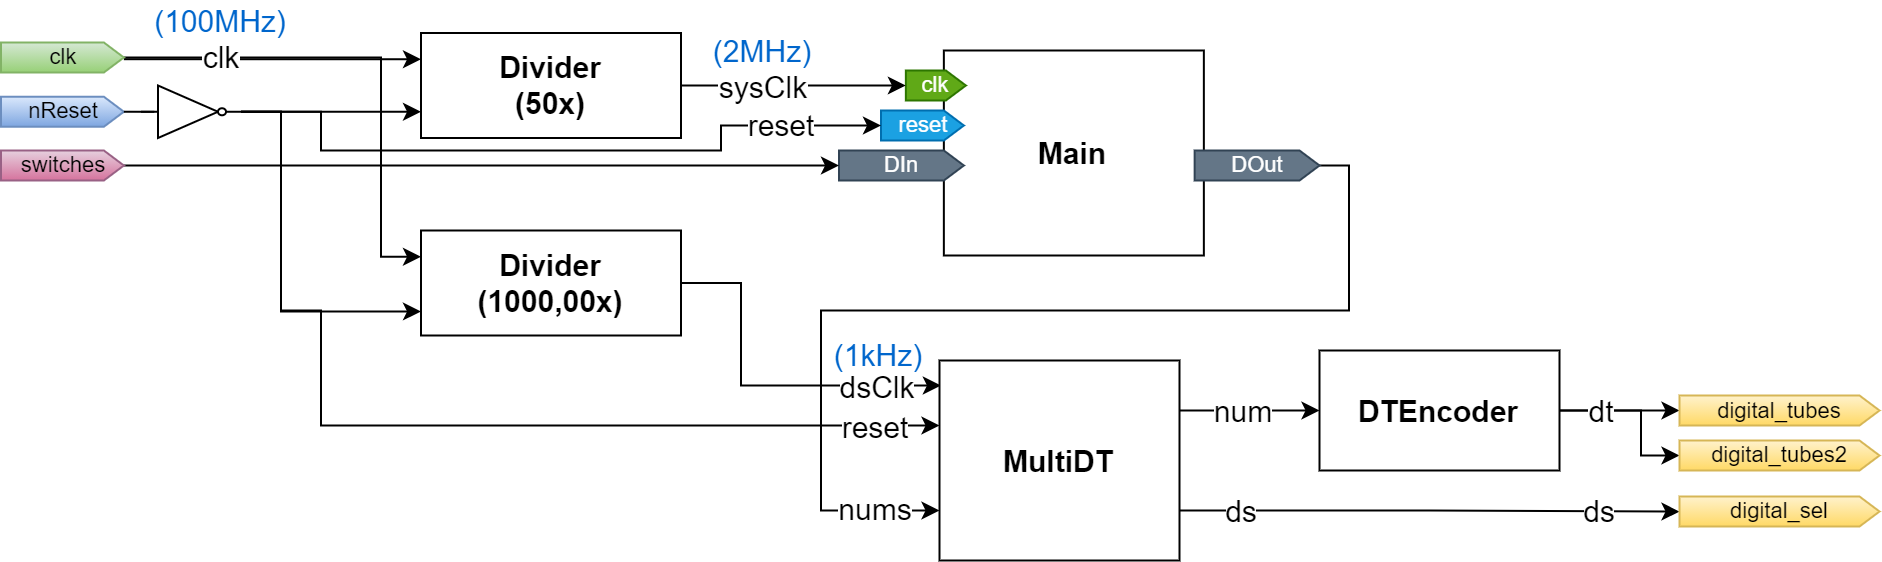
\includegraphics[width=10 in]{images/PCOCD-P4-pratical-block.png}%
	\end{adjustbox}
\end{figure}
\clearpage

\end{document}
